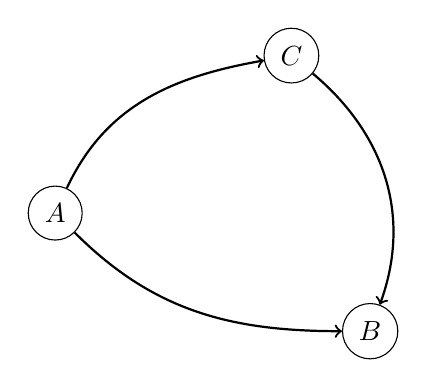
\begin{tikzpicture}[main/.style={draw, circle}]
    \node[main] at (0, 1) (A) {$A$};
    \node[main] at (4, -0.5) (B) {$B$};
    \node[main] at (3, 3) (C) {$C$};

    \draw[->, thick] (A) to [out=65, in=190] (C);
    \draw[->, thick] (A) to [out=-45, in=180] (B);
    \draw[->, thick] (C) to [out=-40, in=70] (B);
\end{tikzpicture}